\documentclass[a4paper]{article}
\usepackage{iemss}
\usepackage[pdftex]{graphicx}
\usepackage[authoryear]{natbib}
\usepackage[labelfont=bf,textfont=sf,labelsep=period]{caption}
\usepackage[english]{babel}
% \RequirePackage{lineno} % for line numbers

\pdfpagewidth=210 true mm
\pdfpageheight=297 true mm

\renewcommand{\rmdefault}{phv} % Arial
\renewcommand{\sfdefault}{phv} % Arial

\bibpunct{[}{]}{;}{a}{,}{,~}

\pagestyle{IEMSSheadings}



\DeclareRobustCommand{\orderof}{\ensuremath{\mathcal{O}}}
\DeclareRobustCommand{\threedi}{3Di }

% Text to appear in the header of the pages
\IEMSShead{Baart et al. / Interactive web based flood modeling}

\graphicspath{{figures/}}
\DeclareGraphicsExtensions{.pdf,.png,.jpg}

\title{Interactive web based flood modeling at country wide scale and planter size resolution.}


% Authors Names and Affiliations:  Two spaces below the title, 10 pt
% Arial, Upper and Lower Case, underline author presenting
% paper and  provide his/her email address


\author{\underline{F. Baart}
  \address[A1]{\it{Deltares,
      Rotterdamseweg
      Delft, The Netherlands (fedor.baart@deltares.nl, arthur.vandam@deltares.nl, gennadii.donchyts@deltares.nl)}},
  J. Ha
  \address[B1]{\it{Nelen \& Schuurmans,
      Zakkendragerssteeg,
      Utrecht, The Netherlands (jack.ha@nelen-schuurmans.nl, martijn.siemerink@nelen-schuurmans.nl)}},
  A. van Dam \addressmark[A1],
  G. Donchyts \addressmark[A1],
  M. Siemerink \addressmark[B1]
}


\begin{document}


\begin{abstract}
  The flooding of rural and urban areas is an increasing hazard to society. Accurate and timely predictions are essential for the water manager to prepare and respond to these hazards.
  Predicting flooding requires a numerical model that represents the physical processes (rain, evaporation, infiltration, overland flow, groundwater flow). This model, fed with measurements, and possible measures, calculates the expected flooding.
  The traditional modelling process consists of a three step process: schematization setup, model running and post-processing, with a total feedback time of hours.  This process is suitable for confirmatory modelling. Most of the time, models are applied exploratory, requiring a different workflow.
  Enabling exploratory modelling requires a shift in utilisation of the modelling instrument. Stakeholders are in control and together evaluate ideas by interacting with the model through a mobile compatible website, supported by the modellers’ expertise. Enabling this type of interactive modelling requires a new level of performance.
  The \threedi platform, in which the new approach was applied, consists of a new flooding and hydrological model (1D/2D) with a corresponding cloud based infrastructure. Applications in rural and urban areas of \orderof(1000km2) at a resolution of \orderof(0.1m) have shown its capabilities for both exploratory and confirmatory modelling.
  The ambition that every component should be at least a 100 times faster than the previous approach, resulted in several advancements, both in the numerical engine and the software that interacts with the user and pushes the data to the web. Here we show advancements in the architecture and model communication.

\end{abstract}
\begin{keyword}
\end{keyword}

\maketitle


\section{Introduction}

The flooding of rural and urban areas is an increasing hazard to society. Accurate and timely predictions are essential for the water manager to be able to carefully plan, design and control the effects of flooding hazard.
For the prediction of these flooding hazards requires a numerical model that represents the physical processes (rain, evaporation, flow, infiltration). This model is fed with measurements from current or historic events. The results of these calculations, the expected flooding, is used for damage estimates, dike design, spatial and emergency planning and for coordinating response efforts. Several challenges required an innovative redesign of both the numerical model and the information infrastructure where it is nested within.


These challenges arise from the movement towards more efficient working methods.
\begin{itemize}
\item \emph{Confirmatory versus exploratory}  \cite{Baart2013}
\item \emph{Passive versus interactive}
\item \emph{Solitary versus social}
\end{itemize}

Other challenges arise from the increased data volumes.
\begin{itemize}
  \item \emph{Measurements}
  \item \emph{Communication}
\end{itemize}



The traditional working method for modelers is to prepare the input of the schematization (grid and input measurements), run a model, wait a while for the model to complete and finally post-process the results. This is working method is suitable for confirmatory modeling (making the best prediction a few days ahead). Most of the questions that people use numerical models for are exploratory.

The traditional working method was also that the modeler was in control. The exploratory approach is often a social process where multiple stakeholders interact and the model is used to test and evaluate ideas. This requires the stakeholders to be in control and not the modeler. The main visualization and interaction method is through a mobile compatible website.

The amount of data involved in preparing the model is rapidly increasing. There is an increase in supply of data caused by the ever growing measurement resolution and spatial coverage. For example the topology of waterbodies at a spatial coverage of a small country are used to determine if the water will find its way into ones neighborhood. The topography and infiltration rate at a spatial resolution of a planter determine if the water will flow to ones backyard or the neighbors.
This resulted in the question how can we design a platform that is suitable for this new modeling approach and meets the corresponding challenges.

The 3Di platform, in which the new approach was applied, consists of a new overland flooding model (1D/2D) and a corresponding infrastructure that has been applied for both exploratory and confirmatory modeling of rural and urban areas at coverages of O(1000km2) at a resolution of O(0.1m).
The advances on a numerical level, by implementing a quad tree structure allowing only the relevant physics to be computed, resulting in an order of magnitude speedup have been previously presented. Here we present the new architecture and it's underlying components, resulting in the advances in model interaction and scalability.
The new multi-tier infrastructure was designed under the following conditions:
Every aspect of the system should be 100 times faster than the previous approach.
The main end user is the water-manager, who is assumed to only know how to use a browser and likes to present realistic looking results.
The modeling should be interactive and social, meaning that multiple people can interact with the same running model at the same time.
The system should be able to run both in private and public clouds. The numerical model should be able to run on a single computer on a supercomputer and in the cloud.
The main interface is a mobile compatible website. The model results are rendered on the client in a html5 web map using both bitmap and vector graphics. The user can interact with the model in several ways, for example by changing properties of hydraulic structures, water levels, discharge locations, rain events. The browser transforms these interactions into messages which are pushed back to the model through websockets. Model results are also pushed to the browser using websockets and on request through a Web Map Service (WMS) extended with time support.
The web application server forwards the websockets messages back and forth between the browser and the model. This application also keeps track of authorization, authentication, user preferences and the social aspects, who is watching which model, who is in control.
The numerical model was adapted to an interactive model by implementing the low level, non invasive BMI interface. This interface makes the numerical model adhere to the Hollywood principle (don't call us, we'll call you): the control of the initialize, update and finalize steps are called from outside of the numerical model. All variables of the model can be accessed through direct or shared memory access, allowing for communication within nanoseconds. The numerical model can be run as a command line executable (for operational runs), in a GUI (for schematization design), as a shared library (for data exchange) and as a message publisher/puller (for interaction). A separate tool generates photo-realistic renderings in 3D stereo for presentation purposes. The messaging publisher module, which works for any BMI compliant model, allows to push results to the browser at a rate of over 20 time per second and a latency of under 50ms.
A provisioning module is used to quickly deploy new updates of models schematization and to scale when more running models or WMS servers are required. Models can run at cloud providers and at the central server. Model schematizations are kept under distributed version control so that updates can be pushed and different versions of the same model can be used.
The new platform has been deployed at several locations in the Netherlands and in Singapore. In preliminary tests we found that the model has skill comparable to previous models. Setting the bar for performance a few order of magnitudes higher resulted in new ideas instead of improved existing ideas. A major part of the platform (model messaging, WMS server) has been released open source because it can also be used with other models. The numerical model is shared within a small community.
By solving the challenges new challenges arise. The new challenges are technical and social. How can we dynamically filter out the most relevant information from the platform as the bandwidth and browsers rendering power of the mobile browsers is limited and varying. The shift towards social and exploratory modeling and away from the modeler "in control" require new best practices. How do we make sure information is used correctly? How "true" is the information perceived?

\section{Method}
\subsection{}
\subsection{}

\section{Results}
\subsection{Numerical model}
\subsection{Architecture}
\subsection{Communication}
\subsection{Visualization}
\begin{figure}[h]
  \centering
  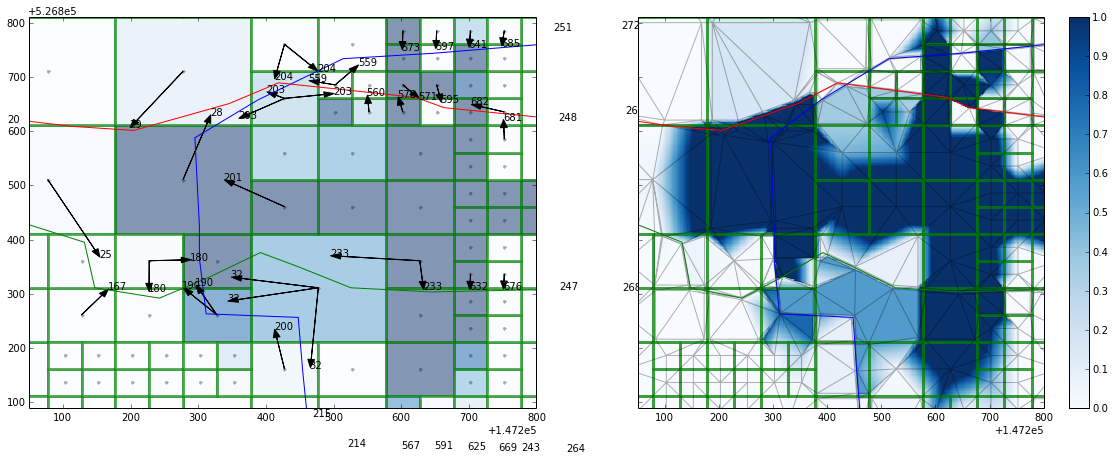
\includegraphics[width=10cm]{interpolationlevees2}
  \caption{Interpolation method}
  \label{fig1}
\end{figure}

\section{Conclusions and Recommendations}




%%%%%%%%%%%%%%%%%%%%%%%%%%%%%%%%%%%%%%%%%%%%%%%%%%%%%%%%%%%%%%%%%
\bibliographystyle{iemss}
\bibliography{bibliography}
%%%%%%%%%%%%%%%%%%%%%%%%%%%%%%%%%%%%%%%%%%%%%%%%%%%%%%%%%%%%%%%%%





\end{document}
